\chapter{Implementation}

The solution, according to the design from the previous chapter, consists of a number of interacting components. To eliminate any possible issues that might happen from integration, all the components were implemented using the same programming language -- Java 8. The solution would be built as a single executable \texttt{.jar} file, with all components bundled into it.

Development was done incrementally -- at the end of each phase the solution would be in a state where it is a working (but incomplete) product on its own. First of all, the battle model was created, with a GUI to test it out. On top of that the AI player was developed. Genetic algorithm can then be applied to optimise the battle systems. Finally, after some adjustments, the solution was adapted into a form suitable for human volunteers to evaluate the resulting battle system.

\section{Phase \rom{1}: manually-controlled battle}

The purpose of the first phase is to build a completely playable game, which requires the complete battle model, the battle controller, and a GUI.

\subsection{Model classes}

Central to the solution is the battle model. The entity classes were put into package \texttt{models} and its subpackage. Relationship among major entity classes are shown in figure \ref{fig:uml_models}.

\begin{figure}
	\centering
	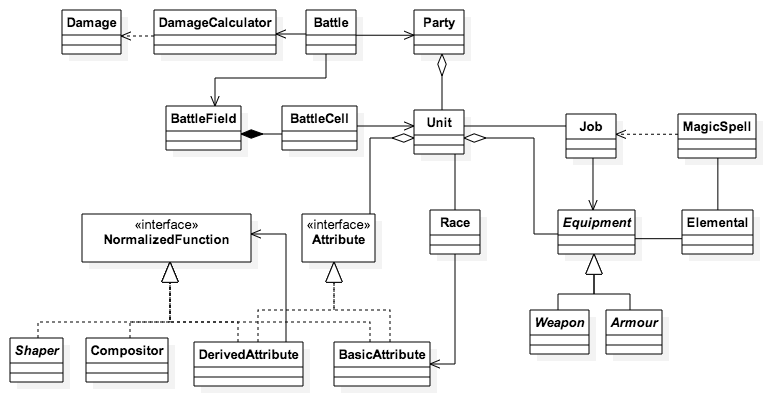
\includegraphics[width=1\linewidth]{figures/uml_models.png}
	\caption{Entity relationship for important model classes.}
	\label{fig:uml_models}
\end{figure}

A subpackage contains parts of the model with sufficient complexity to justify its existence. Notable ones are \texttt{models.equipment}, which contains the models for all weapons and armours, and \texttt{models.calculation} which describes the numerical derivation part of the combat rules.

\subsection{Preliminary battle system}

In this first phase it was not yet necessary to create the full-scale battle system. The calculation, which would later be extracted and parameterised into the battle system, was all fixed at this stage. A few adjustments to the calculation were done manually, just enough to keep the battles from being extremely unbalanced.

As for the derivation functions that map basic attributes to derived attributes, they were also arbitrarily fixed to be one of the following simple shaping functions:
\begin{itemize}
	\item Linear function $f(x) = x$.
	\item Quadratic function $f(x) = x^2$.
	\item Square root function $f(x) = \sqrt{x}$.
	\item The normalized logistic function $f(k, x) = \frac{k^{2x}-1}{(k-1) \cdot (k^{2x-1} + 1)}$, with $k = 10$.\footnote{$f(k, x)$ describes a set of functions $f(x)$ that are results of shifting the logistic function $\frac{1}{1 + e^{-x}}$ to pass through all of the points $(0, 0)$, $(0.5, 0.5)$, and $(1, 1)$.}
\end{itemize}

The battle system would be revisited in phase \rom{3}, where we made it fully configurable.

\subsection{Battle controller}

The battle controller is the centre of communication of the system. The class \texttt{BattleController} implements the behaviour specified in section \ref{sub:battlecontroller} faithfully for the most parts. We made one modification, by adding a loop-breaking condition to the main game loop (previously the game ends only when one side wins). This condition is defined based on the number of turns played in the battle. With this loop-breaking condition, battles that go on for too long can be cut short and declared as being tied. This is to prevent the game from getting stuck in an infinite loop, which could happen in an AI-vs-AI battle that has fallen into an equilibrium.

The battle controller keeps track of the position and timing of all the units. It maintains a \textit{priority queue} that sorts the units by their \textit{action time}, in ascending order. The action time tells when is the next time the unit will get its turn. At the start of the battle, the action time for each unit is initialised to its \textit{charge time} ($\frac{1}{\text{speed}}$). The controller then \textit{let the time progress}, and the unit with the least action time is then selected as the one who gets the next turn. Once the turn is finished, the unit is put back into the queue, with action time equal to the sum of the current time and its charge time.

The model defines an abstract type \texttt{Player}, which has an abstract method \texttt{selectPlay(Unit, List<CommandType>)} that encapsulates the play-selection strategy for each concrete implementation. The controller repeatedly asks the current player to provide the battle actions, updates the battle model accordingly, then notifies the UI and any other interested components about the change.

As stated in the design stage, the notification mechanism was implemented as an event-driven system. We utilised \textit{EventBus}, an annotation-based event handling library which is a part of Google's \textit{Guava} utilities, to do this task. On the event poster side, the following events are posted when triggered by their associated actions:
\begin{itemize}
	\item \texttt{UnitActionEvent}: tells subscribers that a unit has completed an action.
	\item \texttt{DamageEvent}: tells subscribers that an action that can cause damage (including healing -- for convenience we can think of healing as a \textit{negative damage}) is attempted on a unit, successfully or not.
	\item \texttt{UnitDeadEvent}: tells subscribers that a unit is removed from the battle.
	\item \texttt{BattleEndEvent}: tells subscribers that the battle has ended.
	\item \texttt{ActionTargetAreaEvent}: informs subscribers about \textit{target area} -- the set of all possible target cells of a command. For example, when the player chooses the \textit{move} command, this event will tell subscribers about all possible cells that can be the destination of the move.
\end{itemize}

Notice that a single action can cause multiple events. An attack command would generate at least three events, definitely one each of \texttt{UnitActionEvent}, \texttt{DamageEvent}, and \texttt{ActionTargetAreaEvent}. If the attack kills the target then a \texttt{UnitDeadEvent} is also generated. Even a  \texttt{BattleEndEvent} is possible, if the attack kills the last opponent.

\subsection{Random battle generator}

To start a battle, all the pieces of the model need to be instantiated and assembled together. In this phase we only focused on generating random battlefields in a systematic way, whereas everything else was created simply by random selection from finite options.

The design states that the battlefield must be generated in a way that all accessible cells are connected. We added another constraint here: there must be at least 4 accessible cells in the two topmost rows, and at least 4 accessible cells in the two bottommost rows. This is because we want to put the two parties on these rows at the start of the battle, one at the top and the other at the bottom, similar to the starting configurations in chess or checkers. 4 is the maximum number of units in party we used, so at least 4 empty, accessible cells are needed for each party.

The algorithm used to create the battlefield is a variant of the flood-fill algorithm:
\begin{enumerate}
	\item Start with an empty battlefield. Mark the \textit{middle} cell $(\frac{width}{2}, \frac{height}{2})$ as accessible, with an initial height $h_0$. Add the 4 cells adjacent to this middle cell to the \textit{fringe} set.
	\item Randomly select one cell $c$ from the fringe.
	\begin{enumerate}
		\item Mark $c$ as accessible.
		\item Find the set of cells adjacent to $c$ that have already been marked as accessible (at least one exists, otherwise $c$ would not be in the fringe). Randomly pick one of these, and call it $s$.
		\item Set the height of $c$ to either $h_s-1$, $h_s$, or $h_s+1$, where $h_s$ is the height of $s$.
		\item Add all cells adjacent to $c$ that has not been marked as accessible to the fringe.
	\end{enumerate}
	\item Repeat the previous step until the desirable number of accessible cells is reached.
	\item If the number of accessible cells in the two topmost rows or in the two bottommost rows is less than 4, redo the whole process from the beginning.
\end{enumerate}

In simple terms, the algorithm starts from a set of one accessible cell, then repeatedly, randomly expands this set, while maintaining the total-connectedness of all accessible cells.

\subsection{User interface}

\begin{figure}
	\centering
	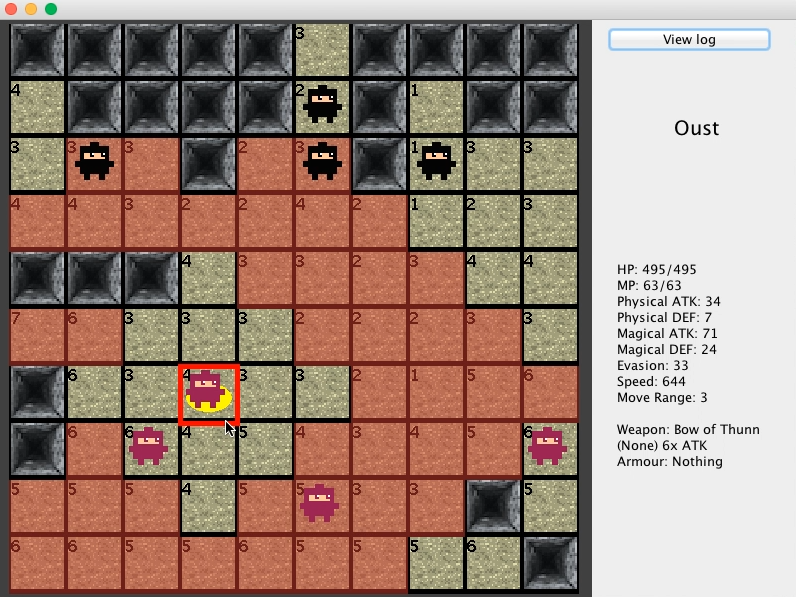
\includegraphics[width=.8\linewidth]{figures/battle1}
	\caption{Battle GUI during phase \rom{1}.}
	\label{fig:guiphase1}
\end{figure}

In this phase, a graphical user interface was implemented as a single-screen Java Swing application, as shown in figure \ref{fig:guiphase1}. This simple GUI allows the battle mechanics to be manually tested. It has the following features:
\begin{itemize}
	\item It displays the battlefield as a 2-D rectangular grid. Accessible and inaccessible cells are distinguished using different background patterns. The height of each accessible cell is written at the top.
	\item Units are displayed on the battlefield using the same sprite, distinguished only by their colours (black or red), to indicate different parties.
	\item Hovering the mouse over a unit will display its statistics (including those of its equipment) in a panel on the right.
	\item A yellow oval is used to indicate the current unit. Clicking on this unit will pop up a menu where battle actions can be selected.
	\item When selecting actions that require a target cell, the eligible cells will be overlaid with a translucent colour (green for move command, red for battle commands). Clicking on one of these cells will commit the command, while clicking outside will cancel.
	\item A log of all actions in the current battle can be viewed by clicking on the \textit{View log} button.
\end{itemize}

For the task of finding the eligible cells, which is not required given the rules of the battle, nevertheless necessary for user experience, the following algorithm is used. It is another variant of breadth-first-search, flood fill algorithm:

Given a starting cell $o$, an adjacency test predicate $adj(c_1, c_2)$, a cost function $cost(c_1, c_2)$, and a maximum cost $C$. 
\begin{enumerate}
	\item Initialise a queue with the starting cell.
	\item Initialise a map $M$ to record the cost of each eligible cell. Set $M[o] = 0$.
	\item Repeat until the queue is empty:
	\begin{enumerate}
		\item Take a cell $x$ out of the queue.
		\item For each cell adjacent to this cell (that is, for every cell $y$ passing the adjacency test $adj(x, y)$), calculate the new cost $nc = M[x] + cost(x, y)$.\footnote{The cost function is usually a uniform function $cost(x, y) = 1$, but different scheme can be applied if the game rule changes.}
		\item If $nc$ is greater than the maximum cost $C$, ignore this cell.
		\item If $M[y]$ is not recorded yet, or if $nc < M[y]$, then set $M[y] = nc$ and put the cell $y$ into the queue. 
	\end{enumerate}
	\item All the keys in the map $M$ are the resulting eligible cells.
\end{enumerate}

\bigskip
At the end of this phase, the program was in a playable state, with random battlefield and units each time a battle was generated. The game was in 2-player mode since the AI did not exist yet. We had no control over how the units were generated, and the battles could be quite overpowered at times, since the mages were very weak in this system. These missing components would be created in later phases.

\section{Phase \rom{2}: automated player}

In this phase, the AI player was introduced. It was implemented as a concrete subclass of \texttt{Player}, called \texttt{SmartPlayer}. It follows the concept of \textit{HP-change potential}, as described in the design in section \ref{sub:aidesign}. Although the strategy involves complex calculation steps, the implementation itself follows the design rather straightforwardly. 

The basic building block of the strategy is the amount of damage (and healing) when a unit makes a certain combat action against a target. Damage calculation, as described in section \ref{sub:dmgcalc}, includes a random variation that makes the actual amount of damage varying in the range of 50\% to 150\% of the base damage. It is also possible for an action to be unsuccessful, depending on the \textit{evasion} attribute of the target. These two factors make the exact amount of damage uncertain. We could have programmed the AI and the battle model in such a way that the AI is an \textit{omniscient agent} -- i.e.\ having full access to the exact outcome of any actions.\cite{russell2010artificial} However it was decided that that would give the AI too much unfair advantage, and the AI should only be allowed to know what can be theoretically known to human players -- which obviously do not include results of randomisation. Instead the AI uses the \textit{expected damage}, calculated simply as the \textit{product of the base damage and the chance of success}, which is $(1 - \text{target's evasion})$. 

The strategy also includes finding the number of moves required for a unit to attack another. There would be a lot of redundant calculations if this is implemented naïvely. Therefore, a cache of the distances (in terms of number of moves required for each unit) between all pairs of battle cells is maintained. These distances are figured out only once using the flood-fill algorithm previously described. Once calculated, they can be reused throughout the battle, thus in the long run this improves the time-efficiency of the AI.

The GUI was extended to let the user select the two players, so the battle can be Human vs Human, Human vs AI, or AI vs AI. We observed the behaviour of the AI, given different values to the configurable weights of each sub-strategy (attacking, healing, or avoiding damage). We found that if avoiding-damage is given too much weight, battles could end as draws very easily, since both parties would prefer to maintain safe distance out of attacking range of the other. Therefore we calibrated the weights so that the AI prefers attacking a little more than healing, and avoiding damage is given very little weight, effectively acting as a tiebreaker only.

At this stage we tested the AI manually, by playing against it, and found that it was competent to a satisfactory degree. It did not make useless moves, and it was capable of winning against us quite often.

\section{Phase \rom{3}: procedural generation of balanced battle system}

In this phase, as we already had a stable battle model and AI, we turned our focus to the battle system development and generation.

\subsection{Full battle system}

The battle system is a collection of configurable parts of the model. In the first two phases, these were embedded throughout the model classes. It would be most convenient and manageable if all the configurations are aggregated together in the same module. The class \texttt{BattleSystem} was created for this purpose. It collects all the configurable parts as public, serializable fields.

As the plan is to eventually generating battle systems using genetic algorithm, the class has to be designed to work in conjunction with \textit{Jenetics}\cite{holzinger2014interactive}, the genetic algorithm framework we will use. Jenetics works on a population of \textit{genotypes} -- structural representatives of the solution -- in this case, a \texttt{BattleSystem} instance. A genotype consists of several \textit{chromosomes}, which in turns consist of several \textit{genes}. For simplicity we conflated the concepts of chromosomes and genes together, by fixing the number of genes per chromosome to 1. Each configuration value then needs to be expressed in terms of chromosomes.

Jenetics provides a few different data types that can be used as a chromosome, therefore a solution can be encoded not only as a \textit{bitstring}, but also as a sequence of integers or floating point numbers. The data type in a single genotype is required to be the same\cite[6]{jenetics-manual}, and we chose \textbf{integers} as the basic building blocks. All the configuration values identified from section \ref{sub:battlesystemdesign} can be classified into four groups:
\begin{itemize}
	\item integers
	\item floating point numbers
	\item derivation functions with a single source
	\item derivation functions with two sources
\end{itemize}
Each of these would need to be converted to one or more integers. Integers themselves obviously need no conversion. For floating point numbers, they are multiplied by 100 and rounded to the nearest integer, therefore preserving the original precision at the scale of 0.01. Derivation functions are more complicated.

\begin{figure}
	\centering
	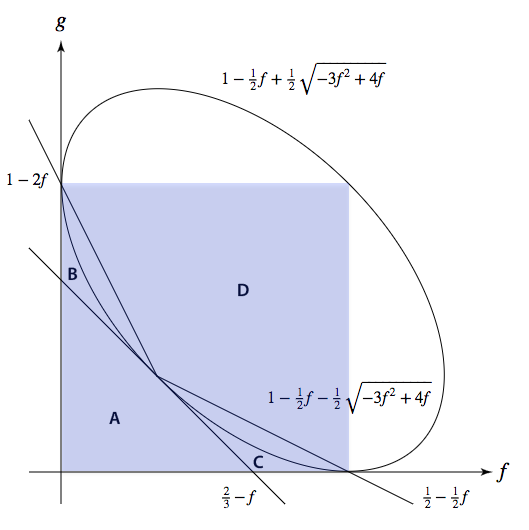
\includegraphics[width=0.7\linewidth]{figures/bezier}
	\caption{This graph shows the eligible area that the other two control points can be placed, when fixing the first and last control points to (0, 0) and (1, 1), that would preserve the monotonicity property of the Bézier curve. The purple square is the area within (0, 0) and (1, 1), which is completely inside the eligible area. (Graph adapted from \cite{web-bezier})}
	\label{fig:bezier}
\end{figure}

In phase \rom{1}, each derivation function was selected from a small set of functions. Here we wanted more flexibility, so \textit{cubic Bézier curves} were chosen in their place. Cubic Bézier curves are parametric curves with 4 control points, often used in computer graphics. They can also be used as shaping functions.\cite{web-flong} By fixing the first ccontrol point to the origin, the last control point to (1, 1), and the other two to be in the unit square, it can be guaranteed that the resulting curve will be a shaping function -- a monotonically increasing function that passes through (0, 0) and (1, 1).\cite{web-flong, web-bezier} Therefore the derivation functions with single source can be encoded as 4 floating points -- 2 points for each unfixed control point, plus another integer for maximum domain value. The floating point numbers are then converted to integers, resulting in 5 integer parameters per derivation function. Derivation functions with two sources use similar conversion process, with another floating point parameter for the weight given to the first source, resulting in 6 parameters per function.

Using the process as outlined above, a battle system can be encoded as a genotype of 96 integers.

\subsection{Battle generator and constraints}

Evaluation of battle systems requires simulating battles in some constrained environment. In this phase the battle generator was extended by allowing constraints to be specified on the units to be generated.

Aside from the battlefield generator which was implemented in phase \rom{1}, the following capabilities were added:
\begin{itemize}
	\item The basic attributes of each unit are still generated randomly, but the average and maximum deviation of these values can be set. The default setup values we used are 0.5 for the average and 0.3 for the deviation, which allow the range of attributes to be [0.2, 0.8].
	\item The material attributes of each equipment can also be constrained in the same way.
	\item The number of units with specific job types can be constrained, using the quota system as described in section \ref{sub:battleeval}.
	\item Races can also be constrained in the same way.
	\item Equipment types are constrained indirectly by the choice of jobs.
	\item A generator can be serialized to a JSON data file.
	\item The whole process is deterministic, meaning that given the same configuration and random seed, the end result will also be exactly the same.
\end{itemize}

The implementation of these features are located in the subpackage \texttt{generators} and \texttt{generators.constraints}.

\subsection{Evaluator and the combined objective}

In the design stage, two major objectives were stated: the combat triangle and the clerics as helpful supporters. We have also added a simple objective named `no first-mover advantage', stating that both parties should have equal chance of winning a random battle. All of these are based on the same principle of evaluation: they were all measurements of win rate for a given situation.

The evaluator takes a battle system and evaluates it against a given objective, with a specified method of combination. The objective would reference all the necessary battle generators. For each generator, AI self-battles will be simulated for a given number of times. The following are collected, by listening to the events issued by the controller:
\begin{itemize}
	\item Raw statistics for each generator, such as the winning percentage of the first team against the second, total runtime, or the average number of turns in a battle.
	\item The fitness of all the objectives at every level.
\end{itemize}

To combine multiple fitness values $V = \{v_1, v_2, \ldots, v_n\}$ together, given weights $w_1, w_2, \ldots, w_n$, and $W = \sum_{i=0}^{n} w_i$, the following options of combination were implemented:
\begin{enumerate}
	\item \textbf{Min-max method}. As our objective is to minimising, this method would simply takes $\min(V)$ as the combined objective. This method ignores the weights.
	\item \textbf{Weighted average}. The combined objective is $\frac{\sum_{i=0}^{n} w_i \cdot v_i}{W}$.
	\item \textbf{Weighted geometric mean}. The combined objective is $  \sqrt[\uproot{3}W]{ \prod_{i=0}^{n} v_i^{w_i}}$.
	\item \textbf{Weighted-normalised geometric mean}. This is similar to the regular weighted geometric mean method, but each sub-objective is added by 1 before taking the geometric mean, to handle the case where one sub-objective has a value of zero, which would render all other sub-objectives irrelevant. The combined objective is then $\sqrt[\uproot{3}W]{ \prod_{i=0}^{n} (v_i + 1)^{w_i}}$.
\end{enumerate}

The evaluator was implemented as both a routine that can be called from another class -- intended to be used by the procedural generation process, and as a command line program.

\subsection{Procedural generation by genetic algorithm}

As planned from the design stage, battle systems are procedurally generated using genetic algorithm. We utilised \textit{Jenetics}, a genetic algorithm framework implemented using the stream concept of Java 8 that promotes parallelization.

The process works as follows:
\begin{enumerate}
	\item A starting \textit{population} of candidate battle systems is created, either from random \textit{genotypes}, or from existing population from a previous run.
	\item Each member of the population is evaluated, using a \textit{fitness function} that calls upon the evaluator.
	\item Standard genetic algorithm operations (selection, crossover, mutation) are applied here to create the next generation of population from the current one. We used the following setup:\footnote{For details of these operations, see the Jenetics manual \cite{jenetics-manual}.}
	\begin{itemize}
		\item \textit{Tournament selection} of size 4 was used for survivors selection. The winner of a round-robin comparison between 4 randomly selected members survives.
		\item Offspring selection was also done using tournament selection, but the tournament size is 3 to reduce the selection pressure. The selected offsprings are then altered, using single-point crossover (swapping two genotypes at a single point) and Gaussian mutator (change a random gene within a genotype to a nearby number).
		\item The survivors and offsprings are combined to form the new generation.
	\end{itemize} 
	\item Repeat steps 2--3 until no improvement has been made for a fixed number of generations.
\end{enumerate}

Since each invocation of the fitness function performs a lot of computation, mainly on the simulation of AI self-battles, it is desirable for the evaluation to be done concurrently, to speed up the process. Jenetics does this by default, using Java's \texttt{ForkJoinPool.commonPool()}, which is considered to be appropriate in most cases.\cite{jenetics-manual} As long as the fitness function is implemented in a thread-safe manner then we can utilise this default setting without any intervention.

Even with multithreading, it still usually took several hours to complete the process from scratch. The evaluation procedure we eventually settled on works like this: the initial run would start from random population using min-max combinator, then the result of this run would be used as starting population for other combinators. This shortened the computation time needed, since the starting point for other methods is usually already producing a good outcome. The result battle system from each combinators are then compared, rather subjectively from game-playing experience, to evaluate which one works best.

\section{Phase \rom{4}: fine-tuning}

The implementation from the previous phase was complete, according to the design. But after running the genetic algorithm engine, it was found that the design was underspecified, and some more work is needed to make the system perform better.

\subsection{The overpowered system}

The first few attempts at generating battle systems produced very good results, measured against the objectives, especially the combat triangle objective. However, after playing those system manually, it was quickly found out that the battles under these systems were extremely short. Most of the attacks were either so powerful the target was killed instantly, or so ineffective that no damage was taken. While these systems are balanced, they are also too overpowered to the degree that the game was unplayable.

The first attempt to remedy this situation was to introduce a new objective that specifies a preference for the length of the game in terms of \textit{total number of turns}, by specifying a target number and evaluate battles to be better when the actual number of turns is closer to the target. More formally, we wanted to minimise the objective function $\frac{|n-t|}{t}$, where $n$ is the actual number of turns and $t$ is the target. It was found that this objective is very difficult to achieve, since all the target values we tried produce results with higher value than the combat triangle objective, as shown in figure \ref{fig:plot_multiobj}.
This objective was then abandoned.

\begin{figure}
	\centering
	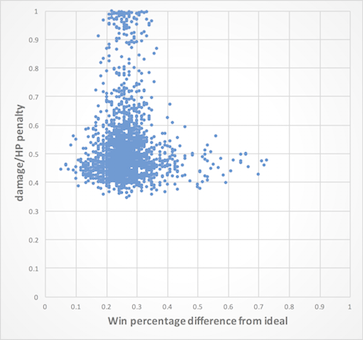
\includegraphics[width=0.6\linewidth]{figures/plot1}
	\caption{A plot of combat triangle evaluation ($x$-axis) against number-of-turn evaluation ($y$-axis), for every individual in all generations of a GA run. The $y$-value plateaus at around 0.35.}
	\label{fig:plot_multiobj}
\end{figure}

The second attempt was to use another objective function based on the size of damage. Damages are classified into 10 bins, based on their relative size to the maximum HP of the target unit, from 0\%-10\%, 10\%-20\%, and so on. Each bin has an associated \textit{penalty} value between 0  and 1, the lower indicating more desirable range of damage. The objective was set up to drive the damage into 10\%-40\% range. We found that this was better than the first attempt, but still difficult to achieve.

It was then suspected that the damage calculation might be too stiff, making it too difficult to optimise. As a result, more parameters were added specifically for this, generalising the \textit{base damage} calculation equation from:
\[
ATK \cdot \frac{ATK}{ATK+DEF}
\]
to:
\[
C_1 \cdot ATK^{C_2} \cdot (\frac{ATK}{ATK+DEF})^{C_3}
\]
The constants $C_1$, $C_2$, and $C_3$ improved the result, but still not to our satisfaction.

The last modification made was on the data collection method, where the percentage calculation was changed from:
\[
\frac{\text{actual damage}}{\text{max HP of the target}}\] to: 
\[
\frac{\text{actual damage}}{\text{average max HP of all units}}
\]
This makes the objective more focused, and easier to achieve. The resulting battle systems are no longer overpowered, while keeping the combat triangle intact.

\subsection{The ineffective black magic system}

Another unexpected result was from a battle system that is well-balanced in terms of the combat triangle, but black magic is surprisingly very weak. Mages do have strong advantage over warriors as specified in the objective, but not as a result of powerful magical attack. This was because the genetic algorithm had adjusted mages' physical attack to be very strong, while totally ignored black magic.

This is not a fault of the genetic algorithm, but rather because the constraints on the system are underspecified. There are implicit constraints that we failed to make explicit. In this case we should have specify that mages should not be able to do more physical damage than magical, or that the physical strength of mages should be less than other classes.

In any cases, the implementation do not have a mechanism to support these constraints, therefore a workaround was used instead: the AI was made to prefer magical over physical attack. At first we simply adjusted the weight of black magic, from about the same as physical attack, to twice higher. This was not effective, and we kept on increasing the weight, to no success. Finally we had to made adjustments to the AI implementation, so that whenever both black magic and physical attack are available, the AI will always choose the former. This solved the problem, so that the solution can produce battle systems that has combat triangle, and the strength of mages are from magical attack.

\subsection{Objective refinement}

Previously in this phase, another objective, the damage percentage, was added. We also realised that the combat triangle and the clerics objective are actually composed of multiple sub-objectives themselves, and the combination method was fixed to unweighted average for both. After this realisation, we had to go back and make radical changes to the implementation. Instead of being flat, single-levelled, objectives are now implemented as a tree-like recursive structure, where a single objective can be either atomic, or composed of other sub-objectives, as depicted in figure \ref{fig:objective_uml}. An objective tree can also be serialize to a JSON file. The final version of our objective tree is shown in figure \ref{fig:objectivetree}.

\begin{figure}
	\centering
	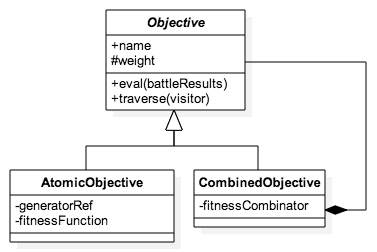
\includegraphics[width=0.7\linewidth]{figures/uml_objectives.png}
	\caption{The classes implementing the recursive objective structure.}
	\label{fig:objective_uml}
\end{figure}

\begin{figure}
	\centering
	\includegraphics[width=1.0\linewidth]{figures/objective_tree.png}
	\caption{The objective tree}
	\label{fig:objectivetree}
\end{figure}

The evaluation command was also adapted and improved as a result of this change. Previously, each sub-objective might refer to the same battle generator (since they share the same battle constraints), and each would generate and simulate the battles separately. This was redundant -- a single round of simulation would be enough for all these sub-objectives to get the necessary information. With this refinement, we had a chance to improve this process, by first collect all the battle generators, run each generator for only a single round, then notify the sub-objectives accordingly.

The objective combinator can be specified for each non-atomic node in the tree. From our subjective evaluation, the min-max combinator works much better than the original unweighted-average to combine the sub-objectives of the combat triangle and the clerics-as-supporters. At the root node we could not clearly identify the best combinator, so we settled for the min-max method as default, but this can be easily overridden from the command line.

\section{Phase \rom{5}: preparation for evaluation}

At the end of the previous phase, the solution could systematically produce battle systems that meet the specified objectives to a satisfactory degree. The next step is to let real players verify that they get the sense of balance from the generated system. The solution needs a few adjustments to prepare for this evaluation step.

\subsection{Recovery of the preliminary battle system}
\label{sub:recovery}

We want to compare the generated system, which is supposed to be well balanced, to another one that is not so. One choice of such other system is the preliminary battle system used back in phase \rom{1}. The implementation of the derivation function had changed a lot from that point -- the fixed set of functions were replaced by cubic Bézier curves. To recover the original system for use in evaluation, Bézier curves that approximate each of the original functions are required. By using numerical methods, the control points in table \ref{table:control_points} (figure \ref{fig:control_points}) were discovered as the ones that provide good approximation, and so the original system was recovered.

\begin{table}
	\begin{tabu}{X[l1] X[c1] X[c1] }
		\toprule
		function & $P_1$ & $P_2$\\ 
		\midrule
		Linear & $(0.5, 0.5)$ & $(0.5, 0.5)$\\
		Quadratic & $(0.333, 0)$ & $(0.667, 0.333)$\\
		Square root & $(0, 0.333)$ & $(0.333, 0.667)$\\
		Logistic & $(0.430, 0.196)$ & $(0.570, 0.804)$\\
		\bottomrule
	\end{tabu}
	\caption{Control points that approximate simple shaping functions}
	\label{table:control_points}
\end{table}

\begin{figure}
	\centering
	\begin{subfigure}{0.24\textwidth}
		\centering
		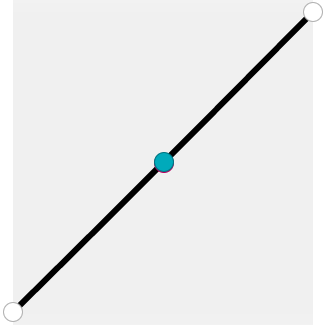
\includegraphics[width=1\linewidth]{figures/approx_linear}
		\caption{Linear}
	\end{subfigure}
	\begin{subfigure}{0.24\textwidth}
		\centering
		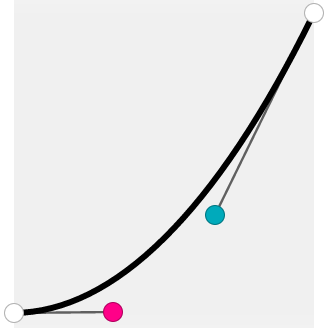
\includegraphics[width=1\linewidth]{figures/approx_quad}
		\caption{Quadratic}
	\end{subfigure}
	\begin{subfigure}{0.24\textwidth}
		\centering
		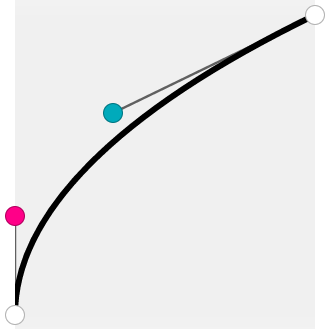
\includegraphics[width=1\linewidth]{figures/approx_root}
		\caption{Square root}
	\end{subfigure}
	\begin{subfigure}{0.24\textwidth}
		\centering
		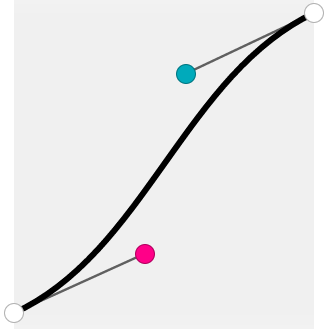
\includegraphics[width=1\linewidth]{figures/approx_S10}
		\caption{Logistic}
	\end{subfigure}
	\caption{Control points and the shape of each approximation of simple shaping functions}
	\label{fig:control_points}
\end{figure}

\subsection{GUI extension}
\label{sub:guiextension}

The GUI had to be extended to accommodate the evaluation process. The following changes/extensions were made:

\begin{figure}
	\centering
	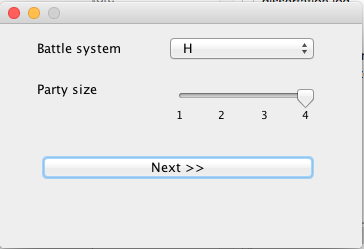
\includegraphics[width=.36\linewidth]{figures/gui_first}
	\caption{Battle system and party size selection screen}
	\label{fig:gui1}
\end{figure}

\begin{figure}
	\centering
	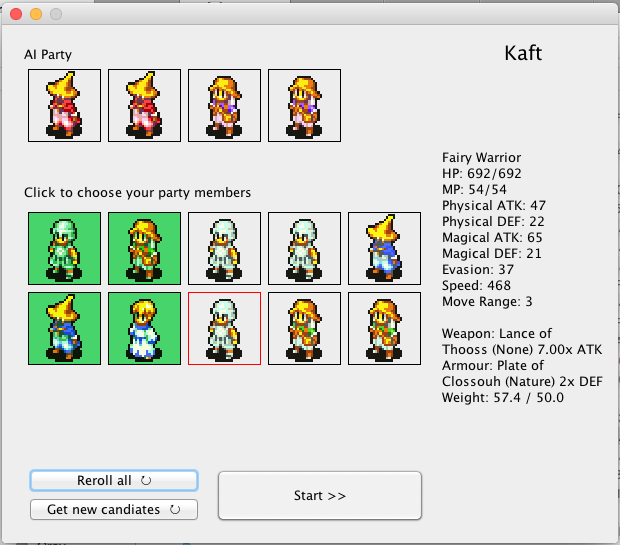
\includegraphics[width=.62\linewidth]{figures/gui_selector}
	\caption{Party selection screen}
	\label{fig:gui2}
\end{figure}

\begin{figure}
	\centering
	
	\begin{subfigure}{1\textwidth}
		\centering
		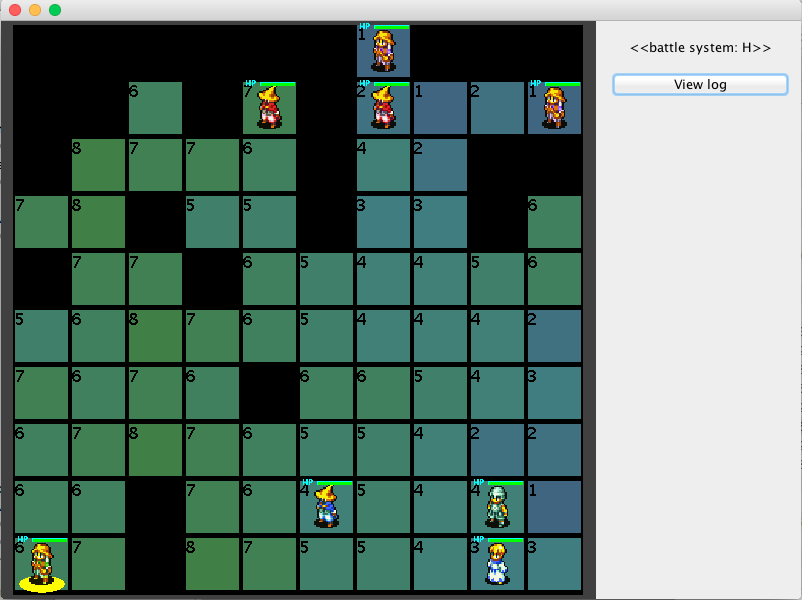
\includegraphics[width=.9\linewidth]{figures/gui_start}
		\caption{At the start of the battle}
	\end{subfigure}
	
	\begin{subfigure}{1\textwidth}
		\centering
		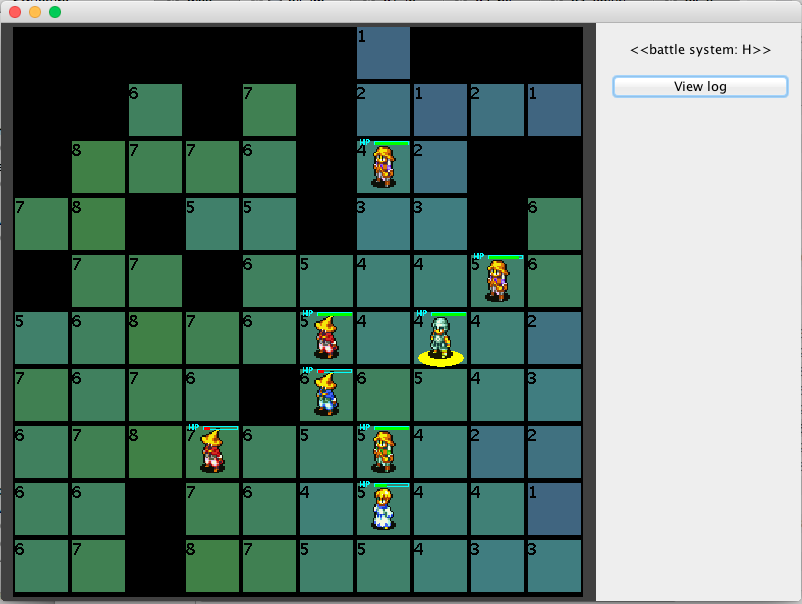
\includegraphics[width=.9\linewidth]{figures/gui_midgame}
		\caption{At the middle of the battle}
	\end{subfigure}
	\caption{Battle screen}
	\label{fig:gui3}
\end{figure}

\begin{itemize}
	\item The interface now consists of three main screens. The first one (figure \ref{fig:gui1}) asks users to pick a battle system and size of the parties.
	\item The second screen (figure \ref{fig:gui2}) shows the AI's party, and 10 units that users can pick to form their party. If the available options are not satisfactory, the users can also hit `reroll' to get a new set of candidates.
	\item The third screen (figure \ref{fig:gui3}) shows the battle, with improved graphical displays. The colour of each cells now provides visual clue to its height. The unit sprites\footnote{The sprites are from the game \textit{Final Fantasy Tactics}. All rights belong to Square Enix.} were changed to make it easier to distinguish between different jobs. There is also an HP bar above each unit, showing its current HP.
\end{itemize}

These changes were mostly small extensions on top of the existing solution. The only exception is the party selection mechanism, which requires generating more units than the party size, thus the battle generator had to be modified. Also, the flow of the program allows users to quit the battle, come back to the party selection, change the members of the party and restart the battle. This raises an issue -- since we used the same model for the units in the selection process and in the battles, if the users quit, then restart the battle, stats like HP/MP that have already been reduced from the previous battle would not be refilled. This was solved by using different copies of the unit instances in the selection process and in the battle. The serialization framework \textit{Kryo} is used for this task, as it enables fast deep-cloning of custom Java objects.

\section{Testing}

Automated test cases were created to ensure the correctness of the implementation, but these are mostly focused on the \texttt{models} module, where most of the calculation happens. Code coverage (measured in terms of number of instructions) for each of the classes in these modules is at least 70\%, as seen in figure \ref{fig:coverage}.

\begin{figure}
	\centering
	
	\begin{subfigure}{1\textwidth}
		\centering
		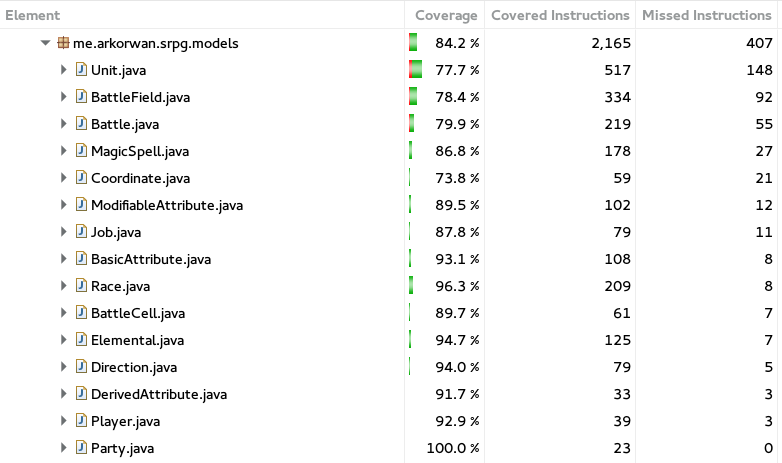
\includegraphics[width=.9\linewidth]{figures/coverage_models.png}
		\caption{The main \texttt{model} package}
	\end{subfigure}
	
	\begin{subfigure}{1\textwidth}
		\centering
		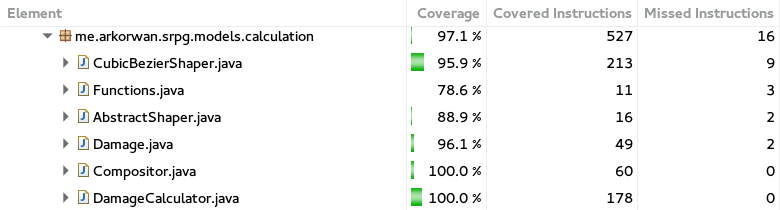
\includegraphics[width=.9\linewidth]{figures/coverage_calculations.png}
		\caption{The \texttt{calculation} subpackage}
	\end{subfigure}
	\caption{Code coverage}
	\label{fig:coverage}
\end{figure}

For other components, manual testing was applied. First, the GUI was manually, exploratively tested after phase \rom{1}, by playing multiple human vs human battles. The AI was tested after phase \rom{2}, by playing multiple human vs AI, and AI vs AI battles, and observing the progress of the game to make sure that the AI did not make any unreasonable choices. The evaluator and genetic algorithm engine were tested by actually run the genetic algorithm, rerun the evaluator on the resulting system to double-check that the results agree, then manually play the resulting system to see if the statistics agree with the actual gameplay.

\section{Challenges and issues}

Throughout the development process there were issues we have encountered. Some were already addressed in phase \rom{4} of the development. This section describes some other notable incidents.

\subsection{Consequences of using EventBus}

EventBus is used in our solution to provide event-based communication between the controller and the subscribers (GUI and the evaluator). It is a convenient solution, but our misuses had caused two related issues:
\begin{itemize}
	\item When an object wants to listen to events, it subscribes to an EventBus instance. The subscriber would then be back-referenced by the EventBus instance, keeping it in the memory until unregistration. One problem we encountered was a memory leak, first observed during the genetic algorithm process, which happened because we failed to unsubscribe evaluators that already finished their work. The leaked evaluator instances would eventually crash the process. The problem was difficult to identify, but easily fixed by adding proper unregistration.
	\item Another problem was that we used a single, centralised EventBus instance for all the battles. When there are multiple battles running concurrently, all the subscribers would get events from all the battles, thus the evaluators would collect more statistics than it should, leading to wrong results. This was fixed by making a dedicate EventBus instance for each battle.
\end{itemize}

\subsection{Deep-cloning of functional interfaces}

As a part of adapting the solution for the evaluation process, unit instances need to be deep-cloned. The serialization framework \textit{Kryo}\footnote{\url{https://github.com/EsotericSoftware/kryo}} is used for this task, as it enables fast deep-cloning of custom Java objects. Most of the elements in the object graph can be cloned without any special handling, except for the \texttt{Compositor} class, which is used to combined two shaper functions into one. This class has a field of type \texttt{DoubleBinaryOperator}, which is a functional interface type introduced in Java 8. Kryo did not handle it as well as other classes, throwing exception when trying to serialize these objects. To solve the problem, these steps have to be followed:
\begin{itemize}
	\item For the functional interface to be serialized (\texttt{DoubleBinaryOperator}), create a new interface (\texttt{SerializableOperator.Binary}) that extends both the original functional interface, and the \texttt{Serializable} interface. Replace the interface to be serialized with this newly created one.
	\item Register a special class to the serializer instance, as follows:
	\begin{lstlisting}[language=Java]
kryo.register(Class.forName("com.esotericsoftware.kryo.Kryo$Closure"), new com.esotericsoftware.kryo.serializers.ClosureSerializer());
	\end{lstlisting}
	The class has to be loaded dynamically by name, since it has been made private by mistake. This has been fixed, and would be included in the next Kryo release\footnote{See the pull request at \url{https://github.com/EsotericSoftware/kryo/pull/415}.}.
\end{itemize}

\section{Summary}

In this chapter, the solution was realised from the design to a concrete program. Most of the implementation sticks closely to the design, but there are some changes along the way, as unforeseen issues were encountered and resolved. At this stage we have a working program that can be used to produce a well-balanced battle system, the quality of which will be evaluated in the next chapter.